% Standalone TikZ source of Fig. 2 (flowchart of Algorithm 1).
% Build the PNG used in the manuscript (run inside figures_src/):
%   pdflatex fig_algorithm_flow.tex
%   pdftoppm -png -r 600 -singlefile fig_algorithm_flow.pdf ../figures/fig_algorithm_flow
\documentclass[border=4pt]{standalone}
\usepackage{amsmath,amssymb}
\usepackage{tikz}
\usetikzlibrary{shapes.geometric, arrows.meta, positioning}
\begin{document}
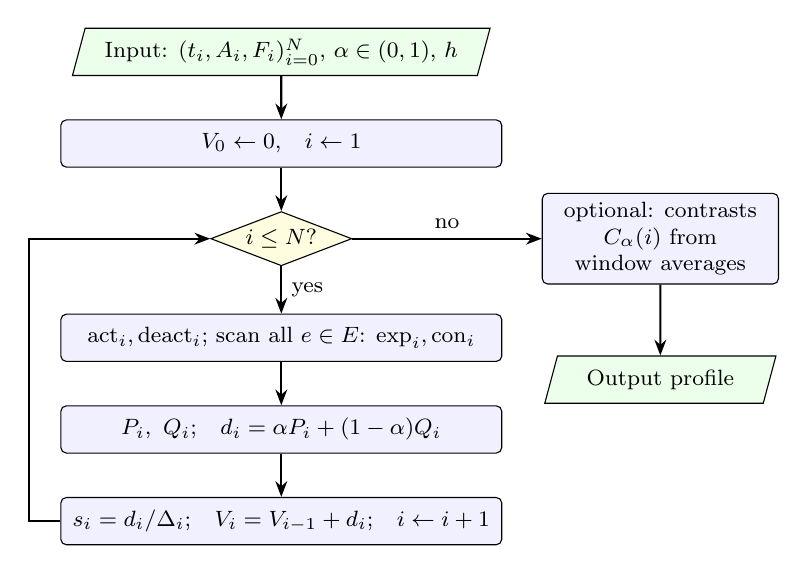
\begin{tikzpicture}[
  node distance=0.55cm,
  box/.style={rectangle, rounded corners=2pt, draw=black, fill=blue!6, align=center, font=\footnotesize, minimum width=5.6cm, minimum height=0.6cm},
  io/.style={trapezium, trapezium left angle=75, trapezium right angle=105, draw=black, fill=green!8, align=center, font=\footnotesize, minimum width=4.5cm, minimum height=0.6cm},
  dec/.style={diamond, aspect=2.6, draw=black, fill=yellow!12, align=center, font=\footnotesize, inner sep=1pt},
  arr/.style={-{Stealth[length=2mm]}, thick}]
\node[io] (in) {Input: $(t_i,A_i,F_i)_{i=0}^N$, $\alpha\in(0,1)$, $h$};
\node[box, below=of in] (init) {$V_0\leftarrow0$,\quad $i\leftarrow1$};
\node[dec, below=of init] (chk) {$i\le N$?};
\node[box, below=0.6cm of chk] (cnt) {$\mathrm{act}_i,\mathrm{deact}_i$; scan all $e\in E$: $\mathrm{exp}_i,\mathrm{con}_i$};
\node[box, below=of cnt] (pq) {$P_i,\ Q_i$;\quad $d_i=\alpha P_i+(1-\alpha)Q_i$};
\node[box, below=of pq] (sv) {$s_i=d_i/\Delta_i$;\quad $V_i=V_{i-1}+d_i$;\quad $i\leftarrow i+1$};
\node[box, minimum width=3.0cm, anchor=west] (win) at ([xshift=0.5cm]cnt.east |- chk) {optional: contrasts\\ $C_\alpha(i)$ from\\ window averages};
\node[io, below=0.9cm of win, minimum width=2.4cm] (out) {Output profile};
\draw[arr] (in) -- (init);
\draw[arr] (init) -- (chk);
\draw[arr] (chk) -- node[right, font=\footnotesize]{yes} (cnt);
\draw[arr] (cnt) -- (pq);
\draw[arr] (pq) -- (sv);
\draw[arr] (sv.west) -- ++(-0.4,0) |- (chk.west);
\draw[arr] (chk) -- node[above, font=\footnotesize]{no} (win);
\draw[arr] (win) -- (out);
\end{tikzpicture}
\end{document}
